\section{Computing the vacuum polarization}
\label{sec:Computing-the-vacuum-polarization}

To be able to compute Eq.~\eqref{eq:vacuum-polarization-long}, some rearrangements are to be done. By use of $-\omega_n = \omega_{-n}$, $\rho$ can be expressed as a single sum
\begin{align}
    \rho = \lim_{\tau \to 0} 
    \sum_{n>0}^{} 
        \left[ 
            (\omega_n - \varepsilon A_0) \lvert \phi_n\rvert^2 
            - (\omega_n + \varepsilon A_0) \lvert \phi_{-n}\rvert^2
        \right]e^{-i\omega_n \tau}
+ \frac{\varepsilon^2}{\pi} A_0 (z).
\end{align}
Although the limit and the sum do not commute (as one used to the mode sum formula might expect), if the coefficients of the sum decay fast enough, the limit and the sum indeed commute\marginnote{Who wrote this??}. After  commuting, the sum is cut off at some finite mode $N$, which induces oscillations of frequency $\Delta z = \frac{1}{N+1}$. These oscillations are an artifact of the cut off, which must be averaged out. 


\begin{figure}[t]
    \centering
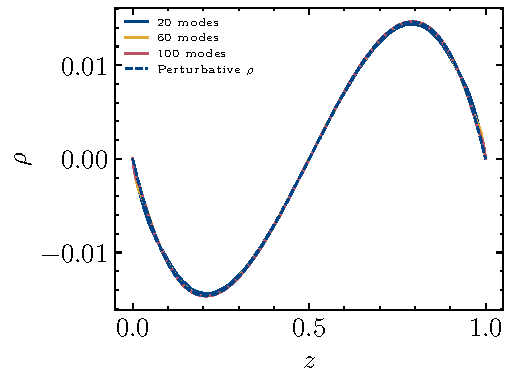
\includegraphics[width=0.8\textwidth]{Figures/dirichlet/unfilteredRhoaa.pdf}
    \caption{$\rho$ of the massless complex scalar field subject to a constant background electric field of strength $\lambda = 1$, for different mode cut-offs, as indicated in the legend. For reference, the perturbative vacuum polarization is given.}
    \label{fig:unfiilteredRhoaa}
\end{figure}
To achieve this, a low-pass filter is applied to the unfiltered vacuum polarization, by convoluting it with a normalized gaussian function, of approximately 3 oscillations of width. The $\rho$ resulting from the filtering is displayed in Fig.~\ref{fig:unfiilteredRhoaa}, where the filtering has been applied to the vacuum polarization resulting from different mode cut-offs (20, 60 and 100, as indicated by the legend). For reference, the vacuum polarization calculated from perturbative theory as per \cite{Wernersson:2020xeh} is also given.
